\section{Background: Simulations, Shadows, Twins}\label{sec:background}

\begin{figure}
    \centering
    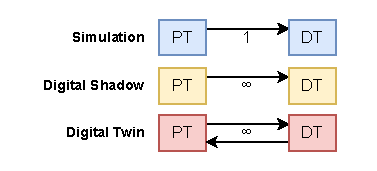
\includegraphics[width=0.75\linewidth]{report/figures/background.pdf}
    \caption{High-level overview and comparison on physical twin (PT) and digital twin (DT) interaction in simulation, digital shadowing, and digital twinning.}
    \label{fig:background}
\end{figure}

In this section, we present background on datacenter simulation, digital shadowing, and digital twinning, and a high-level comparison between these operational techniques illustrated by \Cref{fig:background}.

\textit{``Simulation is defined as the imitation of the operation of a system or real-world process over time, and in many cases, manufacturing provides one of the most important application of simulation"}~\cite{DBLP:conf/wsc/LeeMS03, nicolae5377101m3sa}. Simulation provide datacenter stakeholders with operational insights on infrastructure under workload~\cite{nicolae5377101m3sa}. The top third of~\Cref{fig:background} illustrates simulation as a unique-state prediction task of the physical twin under a simulation scenario. Simulators use \textit{predictive models}, empirical prediction systems that analyze, combine, and compute various input elements to produce fine-grained output predictions~\cite{modsim:book/ZaraiN15:orig, nicolae5377101m3sa}.

\textit{``A Digital Shadow is a set of temporal data traces and/or their aggregation and abstraction collected concerning a system for a specific purpose with respect to the original system.}~\cite{Braun2023_DigitalShadowDefinition}. The middle third of~\Cref{fig:background} illustrates a digital shadowing system which, unlike the single-event of simulation, the digital twin component continously mirrors the physical twin and optionally tracks the state of the physical twin over time.


\textit{``A digital twin is an integrated data-driven virtual representation of real-world entities and processes, with synchronized interaction at a specified frequency and fidelity."}~\cite{DTC_Digital_Twin_Definition_2025}. The bottom third show of~\Cref{fig:background} illustrates the continuous interaction loop between the physical twin, which communicates telemetry data to the digital twin; the digital twin, aided by simulation, suggests SLO-oriented adjustments to the physical twin.

Simulation enables fine-grained datacenter operational monitoring used by stakeholders in decision-making processes~\cite{nicolae5377101m3sa}. \textit{Workloads} contain tasks operated on \textit{infrastructure}, which includes physical machines, virtual machines (VMs), and containers~\cite{nicolae5377101m3sa}. Traces represent recordings or real-world events capturing detailed operational data of the infrastructure under given workload(s)~\cite{nicolae5377101m3sa}.
% Further
% Paragraph on terminology (workload, traces, etc)

% \begin{figure}[t]
%     \centering
%     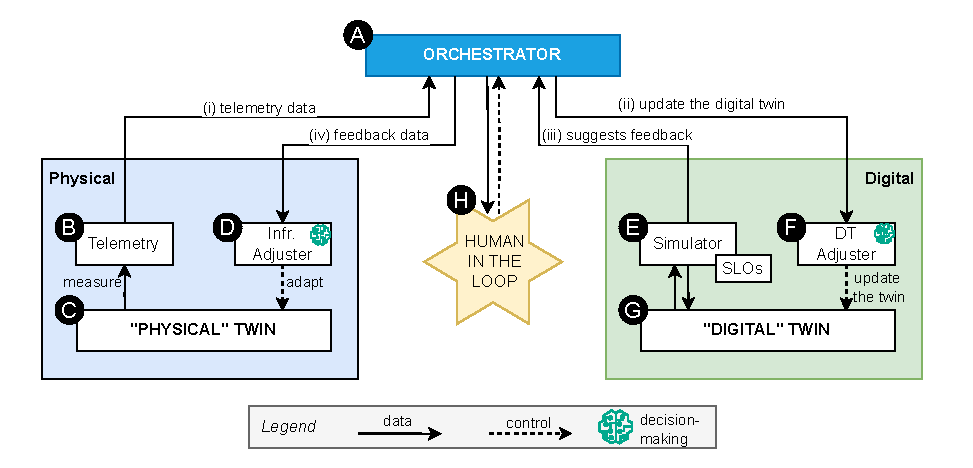
\includegraphics[width=\linewidth]{report/figures/DT-reference-architecture.pdf}
%     \caption{Caption}
%     \label{fig:placeholder}
% \end{figure}


% ======================================
% IMPORTANT - DO NOT DELETE
% IMPORTANT - DO NOT DELETE
% IMPORTANT - DO NOT DELETE


% \subsection{Reference Architectures}

% \subsubsection{Cardiology}

% Recent surveys converge on a layered architecture for digital cardiovascular twins. Data acquisition and integration fuse multimodal streams (wearables and home sensors, ECG/PPG, cardiac imaging, laboratory tests, and EHR), providing a continuously synchronized patient state. In addition to this, domain models combine multiscale cardiac physiology (electrophysiology and hemodynamics) with data assimilation to personalize parameters and quantify uncertainty, while learned surrogates accelerate interfence for clinical workflows based on time. The analytics and decision support then deliver the prognosis, the optimization of therapy and the 'digital trial' of scenarios through clinical interfaces governed by validation, traceability and privacy policies \cite{sel2024building}\citationsneeded{2}.

% \todoall{COMPARE RA \cite{sel2024building} to OPENDT fig or table}

% \subsubsection{Water Systems}

% For water distribution, reference designs resolve around a cyberphysical loop: telemetry via SCADA (pressures, flows, pump/valve states) and network metadata feed a hydraulics backbone augmented with learning-based estimators for partially observed systems; anomaly and change detection trigger model evolution; and operator dashboards translate insights into pump scheduling, valve manipulation, and maintenance priorities \cite{DBLP:conf/isola/DegelerYKLLTT24}\citationsneeded{2}.

% \todoall{COMPARE RA \cite{DBLP:conf/isola/DegelerYKLLTT24}  to OPENDT fig or table}